\documentclass{amsart}
\usepackage{amsmath}
\usepackage{amssymb}
\usepackage{graphicx}
\newcommand{\me}{
    \author{Abhay Shankar K: cs21btech11001}
    \maketitle
}
\begin{document}
\title{Assignment 3}
\me

\begin{itemize}
    \item For all the following graphs, the thread sleep time is an exponential random variable with mean 10ms.
    \item The output file \texttt{output.txt} contains each CS request, entry and exit, along with the times measured relative to the start of the process.
\end{itemize}

\section{TAS} 

\begin{itemize}
    \item Worst case and average diverge due to unbounded waiting
    \item Average time low because of OS scheduling. 
    \item Some average times less than the input average becuase of multiple cores.
\end{itemize}
\centering
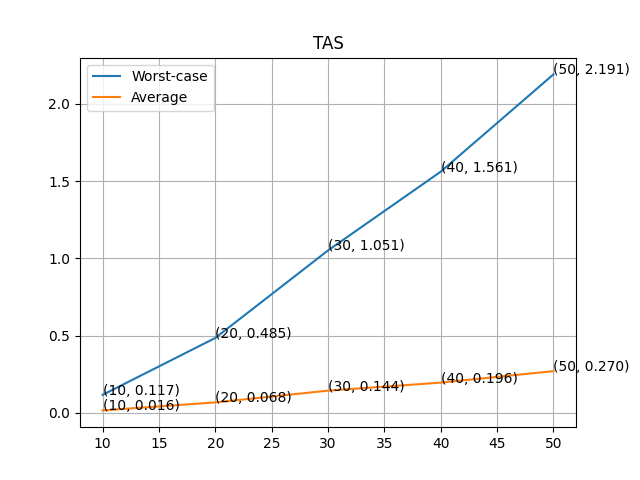
\includegraphics[scale = 0.75]{tas.png}

\newpage

\section{CAS} 

\begin{itemize}
    \item Worst case and average diverge due to unbounded waiting
    \item Extremely low waiting time due to CPU optimizations.
\end{itemize}
\centering
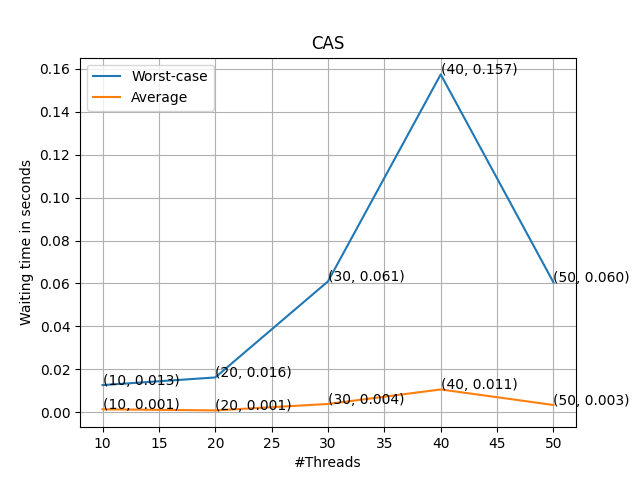
\includegraphics[scale = 0.75]{cas.png}

\newpage

\section{BCAS} 

\begin{itemize}
    \item Worst case and average do not diverge due to bounded waiting
    \item However, waiting time is much higher than others because the thread receiving ownership of the lock may be swapped out.
    \item Alternatively, the scheduler may, through aging etc., ensure some semblance of boundedness in the other two far more efficiently than the manual implementation in BCAS.
\end{itemize}
\centering
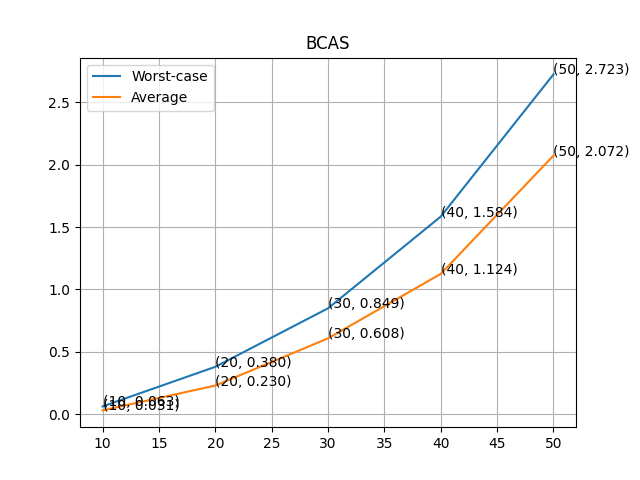
\includegraphics[scale = 0.75]{bcas.png}

\newpage

\section{Average}

\begin{itemize}
    \item The average time for BCAS is much higher, due to aforementioned reasons. 
    \item TAS and CAS have nearly identical graphs, due to similarity of internal implementation.
\end{itemize}

\centering
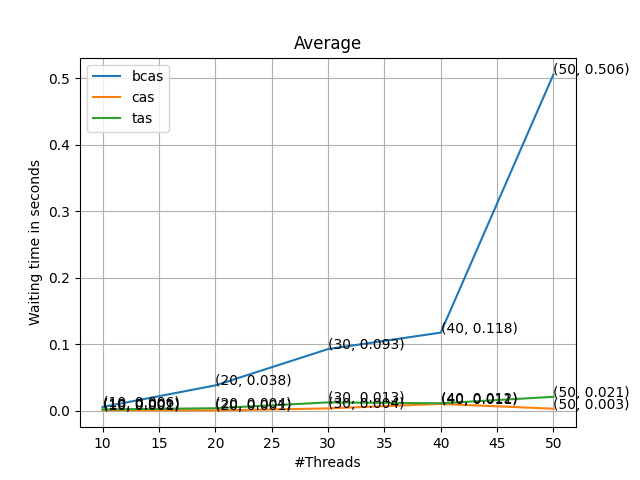
\includegraphics[scale = 0.75]{avg.png}

\newpage

\section{Worst-case}

\begin{itemize}
    \item For CAS and TAS, the worst-case is \(\sim 10 \times\) the average, since the sleep duration is exponential.
    \item For BCAS, due to naive scheduling, the bottleneck is the thread polling and not the critical section itself, so the average is much closer to the worst-case.
\end{itemize}

\centering
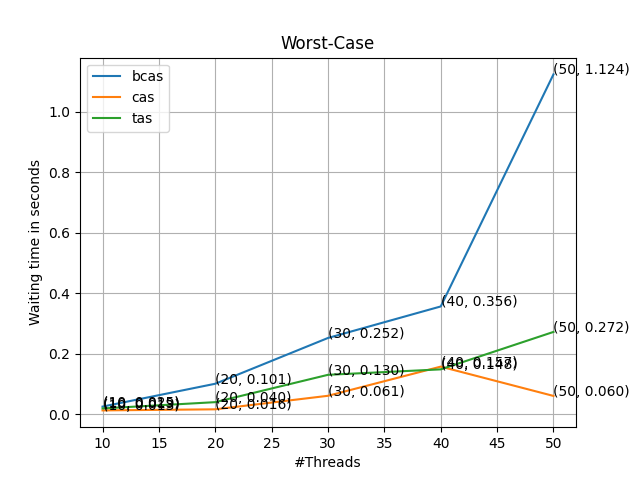
\includegraphics[scale = 0.75]{wc.png}

\end{document}